\documentclass[a4]{report}
\renewcommand{\thesection}{\arabic{section}}
\usepackage[utf8]{inputenc}
\usepackage[brazilian]{babel}
\usepackage{csquotes}
\usepackage[natbib]{biblatex}
\usepackage{booktabs}
\usepackage{outlines}
\usepackage{graphicx}
\usepackage{datetime2}
\addbibresource{bibs/bibliografia.bib}
\addbibresource{bibs/bibdoslivrosesas.bib}
\addbibresource{bibs/standards.bib}
\newcommand{\othersize}{0.7\linewidth}
\usepackage{indentfirst}
\usepackage{caption}
\captionsetup{font={footnotesize,bf},justification=centering,margin=1cm}
\usepackage{subcaption}
\usepackage{hyperref}

\title{Software Project Canvas v1.0}
\author{Geraldo Xexéo}
\date{\today \ \DTMcurrenttime }
\begin{document}

\maketitle

\begin{abstract}
\hspace*{\parindent}Esse artigo apresenta o Software Project Canvas, uma ferramenta ágil que facilita a colaboração das partes interessadas na  discussão e definição inicial de um projeto de software.

Para a sua  criação foram observadas \ref{problems:total} dificuldades  ao ensinar ou utilizar o \textit{Project Model Canvas} no contexto de projetos de software.

As modificações feitas visam facilitar a explicação e o uso de um canvas no planejamento inicial de um projeto de desenvolvimento de software, além de evitar perda de tempo, durante a reunião de concepção do projeto, com discussões semânticas sobre o significado das coisas que não adiantam a definição do projeto.
\end{abstract}

\tableofcontents
\listoffigures

\newpage

\section{Introducão}

Esse artigo apresenta o Software Project Canvas (SPC), representado na Figura \ref{fig:spc}, uma ferramenta ágil cujo objetivo é facilitar a colaboração das partes interessadas na  discussão e definição inicial de um projeto de software.

\begin{figure*}[hbt]
    \centering
    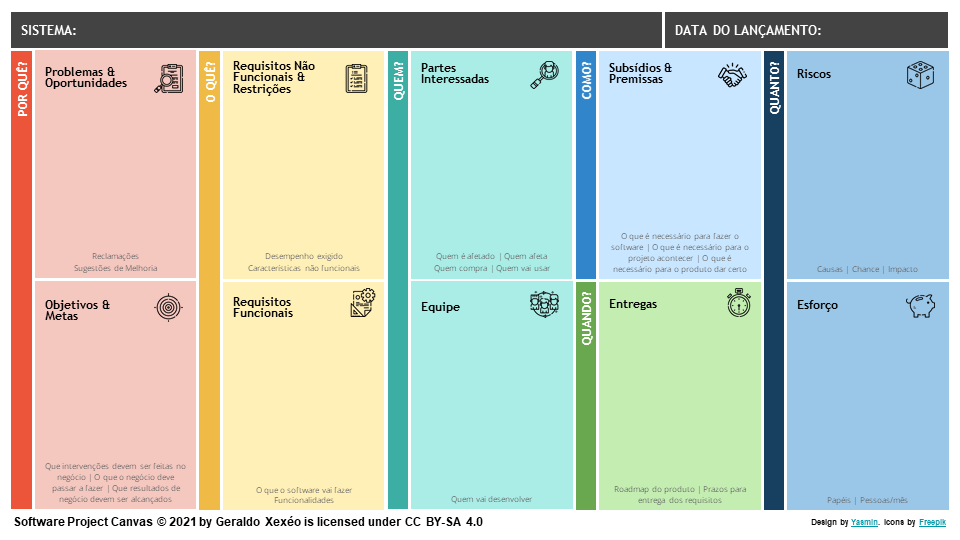
\includegraphics[width=\textwidth]{imagens/Software Project Canvas Yasmin 1.png}
    \caption{O Software Project Canvas. Imagem do autor}
    \label{fig:spc}
\end{figure*}

O \textit{Software Project Canvas} foi motivado por certas dificuldades em ensinar e usar o \textit{Project Model Canvas} no contexto de Engenharia de Sofware. Após identificar essas dificuldades, foram feitas propostas de correção, e variações do modelo foram avaliadas por alguns especialistas e iniciantes na área. 

O artigo contém 6 seções. A próxima seção apresenta o que são canvas, a terceira seção explica a relação entre projetos, agilidade e o uso de canvas, terminando com uma breve descrição do Project Model Canvas. A quarta seção apresenta a proposta do Software Project Canvas, e a sexta seção apresenta a conclusão.

\section{O que são Canvas}

Canvas são ferramentas colaborativas que servem de ponto focal em uma atividade onde algo vai ser, controlado, decidido ou planejado. São compostos de um quadro branco dividido em várias áreas, cada uma representando uma pergunta, assunto ou tópico em discussão, onde são colocados \textit{post-its} contendo a informação desejada. 

Alguns autores\citep{finocchio:2013} associam os canvas a neuro-ciência, tanto por usar de características de agrupamento e proximidade que auxiliam a compreensão dos conceitos, como por apoiarem uma atividade colaborativa que tende a criar engajamento nos membros da reunião em torno do assunto.

O primeiro canvas de grande impacto na indústria foi o \textit{Business Model Canvas}, proposto por \citet{osterwalder2010business}, apresentado ainda vazio na Figura \ref{fig:bmc}. Ele é destinado ao planejamento de um modelo de negócio para um empreendimento. Nele, cada área receberá, em uma ordem pré-estabelecida e ao longo de uma reunião facilitada, \textit{post-its} que dão respostas as perguntas indicadas nos quadros. Por exemplo, no quadro ``Customer Segments'' pode aparecer um \textit{post-it} onde está escrito ``adolescentes praticantes de Skate''.

A partir do sucesso do \textit{Business Model Canvas},  outros canvas foram propostos por pesquisadores, consultores ou pessoas interessadas em algum problema específico. No Brasil, \citeauthor{finocchio:2013} propôs, com bastante sucesso, o \textit{Project Model Canvas}\citep{finocchio:2013}, que serviu de inspiração para nossa proposta. 

\begin{figure}
    \centering
    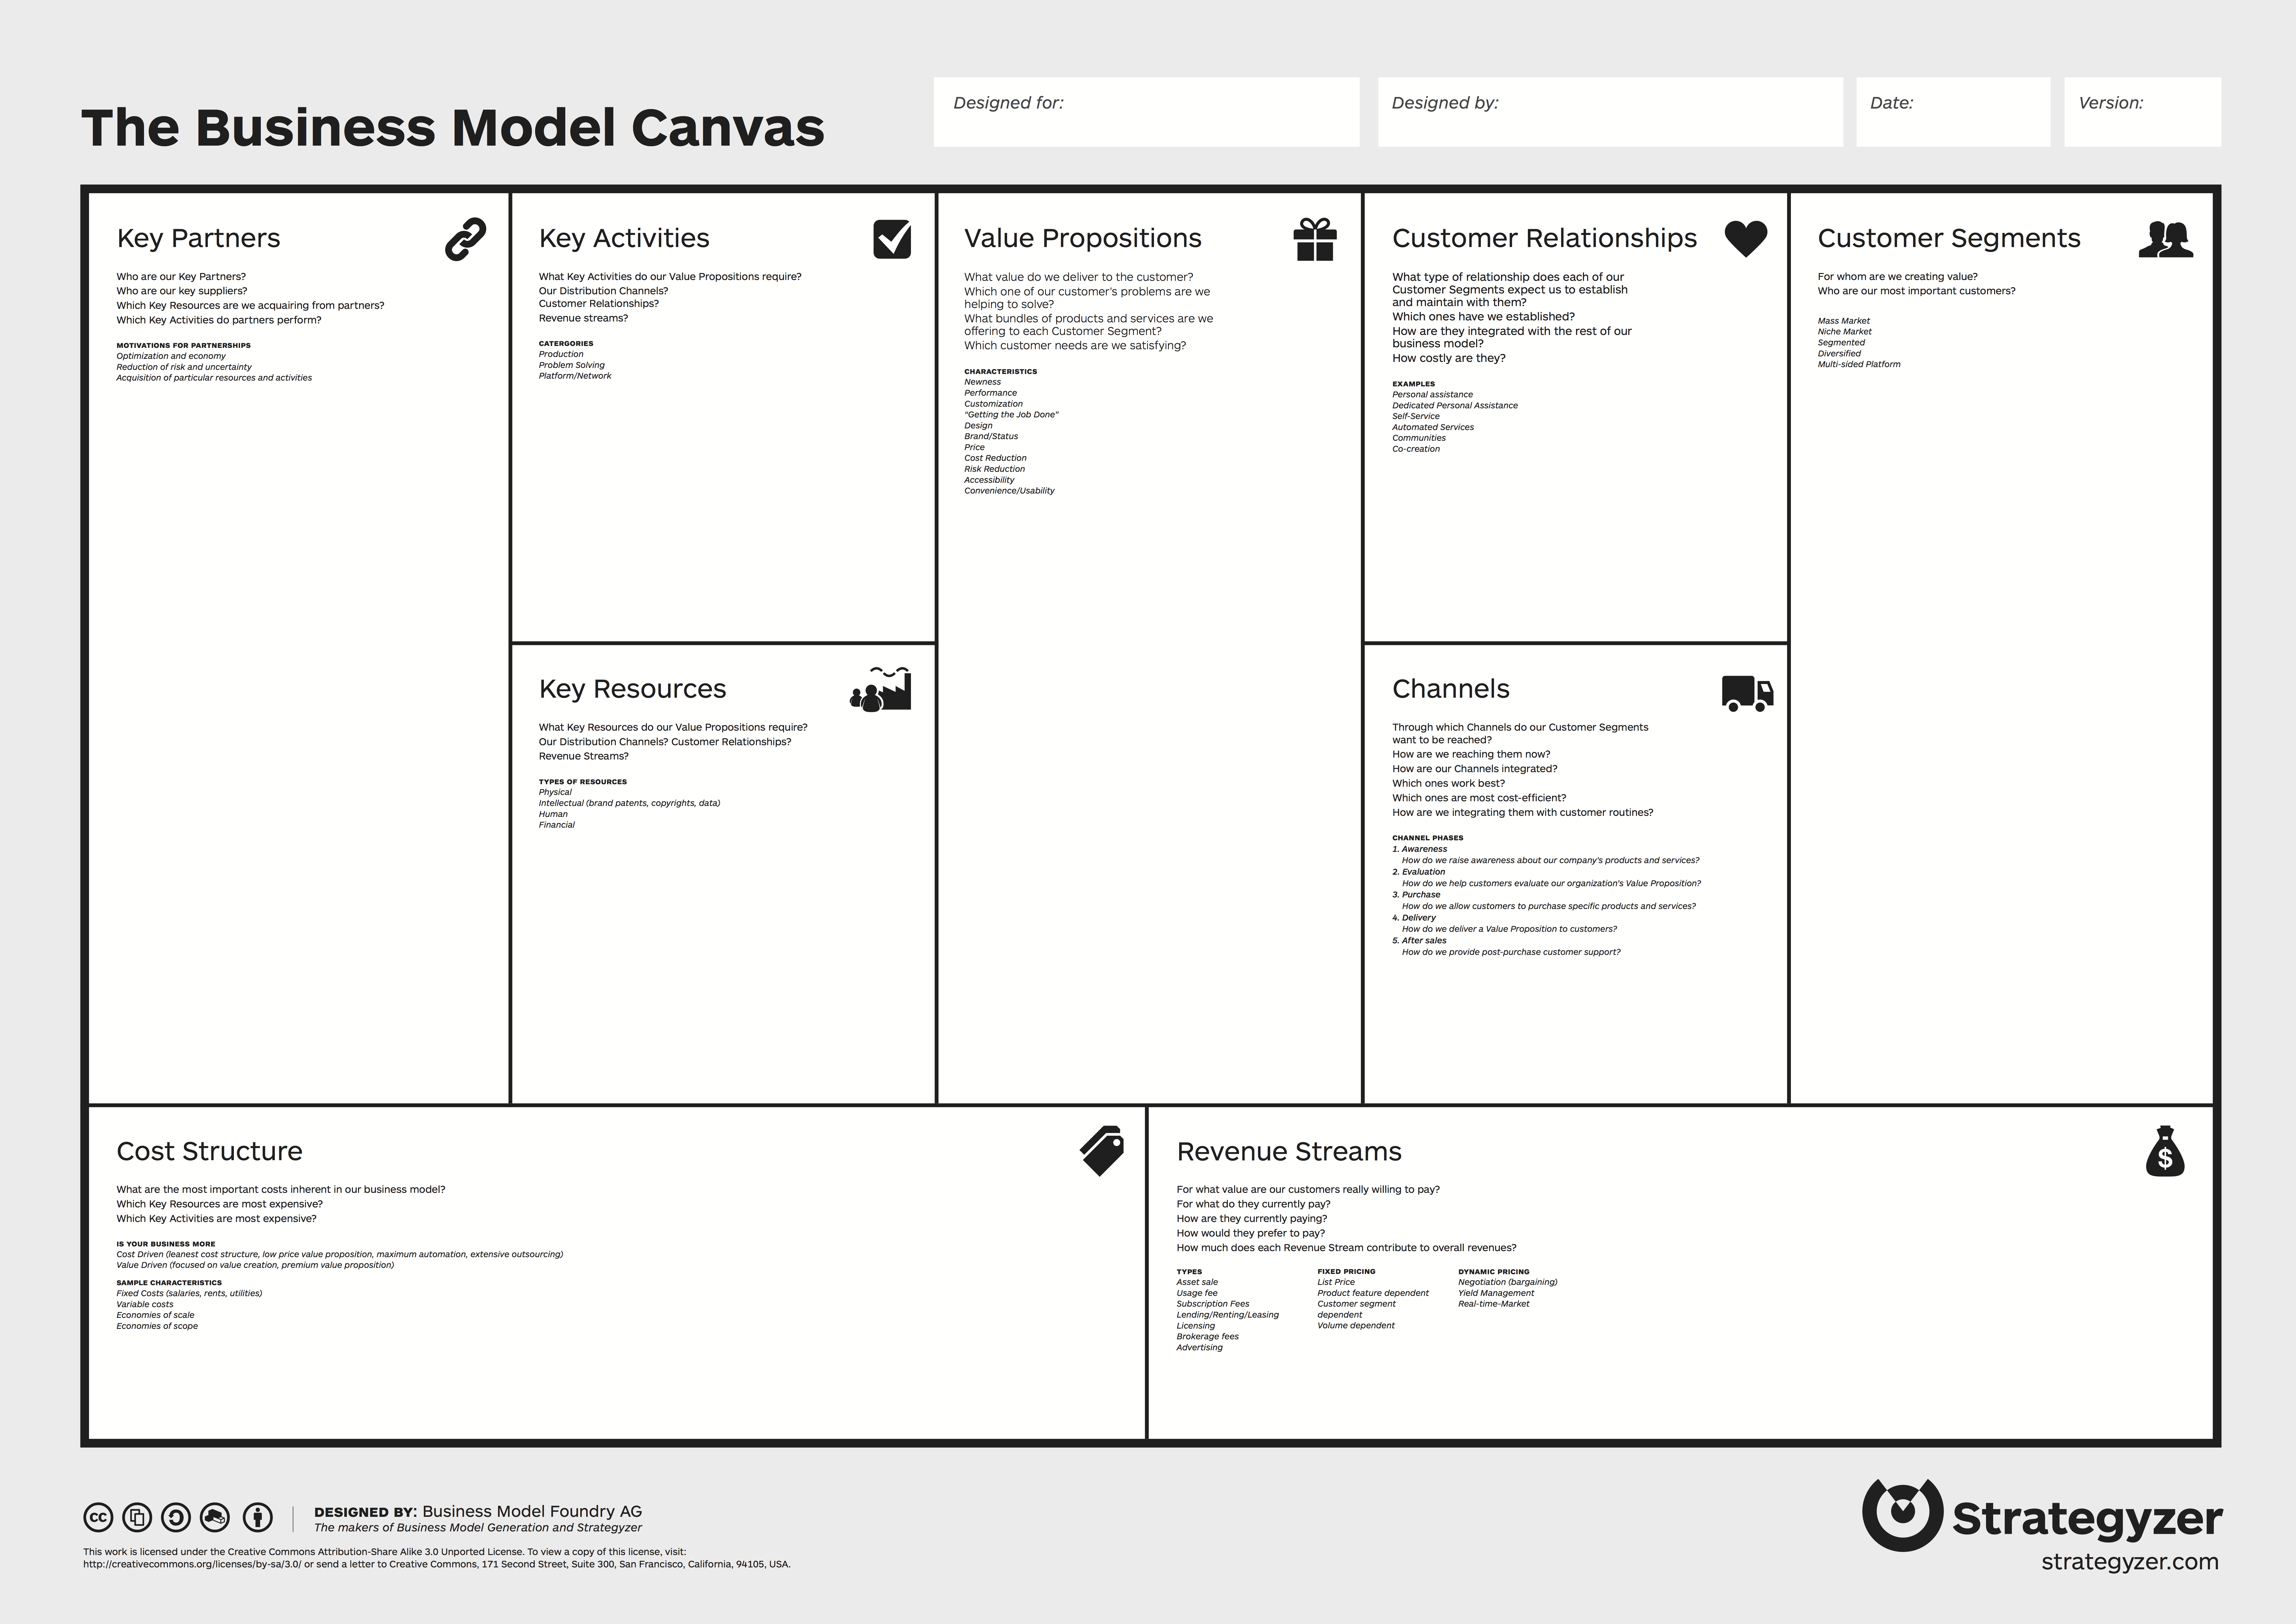
\includegraphics[width=\othersize]{imagens/BMC.png}
    \caption{O Business Model Canvas. Fonte: \citet{osterwalder2010business}}
    \label{fig:bmc}
\end{figure}


\section{Projetos, Agilidade e Canvas}

A Gestão de Projetos é uma área de conhecimento essencial ao sucesso de um projeto. Segundo \citet{kerzner:12ed}, um projeto tem sucesso se 
acaba no prazo, dentro do orçamento, com o desempenho especificado, aceito pelos clientes e usuários, com mudanças mínimas no escopo acordadas entre as partes interessadas, sem causar distúrbio ao fluxo de trabalho da organização e, quando desejado, sem mudar a cultura da organização. Além disso, é necessário satisfazer as partes interessadas\citep{pmbok:6}. Para alcançar todos esses objetivos é necessário planejar, monitorar e controlar o projeto ao longo de sua realização.

Ao longo dos anos, a área de gestão de projetos desenvolveu processos eficazes e reconhecidos, sendo que muitos foram consolidados em padrões ou livros de referência \citep{pmbok:6,kerzner:12ed}. A Engenharia de Software, disciplina relativamente nova em relação as outras disciplinas onde esses processos foram desenvolvidos, foi criada com o intuito de aplicar as práticas de Engenharia ao desenvolvimento de software, incluindo as práticas de gestão\citep{naur:randell:1968,pressman:2019,ieee_computer_society_guide_2014}.

Com a experiência de desenvolver software sob a pressão do mundo de negócios, algumas dessas práticas, ou seus princípios,  começaram a ser contestadas por não serem adequadas ao desenvolvimento de software, exigirem uma carga muito alta de trabalho adicional (\textit{overhead} alto), ou exigirem muitos documentos. Isso resultou no fortalecimento dos defensores de processos de desenvolvimento de software mais leves, que acabaram sendo nomeados métodos ágeis ou enxutos. Essa mudança acabou por afetar toda a indústria, como mostra a ampla adoção dos métodos ágeis e enxutos por outras áreas. 

Entre os princípios que não funcionaram na Engenharia de Software está o da execução de projetos de forma sequencial, onde uma fase é realizada de forma completa e fornece subsídios para a próxima fase, sendo a entrega feita, em sua totalidade, no final do projeto, o que é conhecido como Processo em Cascata. Atualmente, há ampla convicção que é essencial usar processos iterativos e incrementais, onde as entregas são pequenas e feitas ao longo do projeto, principalmente devido a sua maior taxa de sucesso\citep{pressman:2019,chaos:2015}.

Uma prática comum dos métodos ágeis é o uso de quadros brancos com áreas delimitadas por assunto, indicando, de forma transparente a todos, alguma informação controlada  por meio do quadro. O mais famoso desses quadros é provavelmente o a adaptação, para o processo \textit{Scrum}\citep{scrum:sbok:guide}, do \textit{Kanban}, apresentado em uma forma simplificada na Figura \ref{fig:kanban}. O Kanban é um método de produção que pode ser considerado um predecessor dos métodos ágeis e faz  parte de um conjunto de práticas utilizadas na Toyota e que iniciou uma revolução de conceitos de produção e qualidade, alterando o até então paradigma \textit{Fordista} de produção\citep{gross:2003:kanban}. Outros métodos adotaram quadros semelhantes, como o SEMAT \citep{jacobson_essentials_2019}, que usa cartas pré-definidas posicionadas no quadro para indicar o estado de um processo. 

Na Figura \ref{fig:kanban} também é possível notar que o quadro não precisa ser feito de forma impressa, podendo ser simplesmente desenhado em um quadro branco, ou mesmo na parede com fitas, e como os \textit{post-its} são usados, nesse caso para indicar tarefas a fazer, sendo feitas e prontas.

\begin{figure}
    \centering
    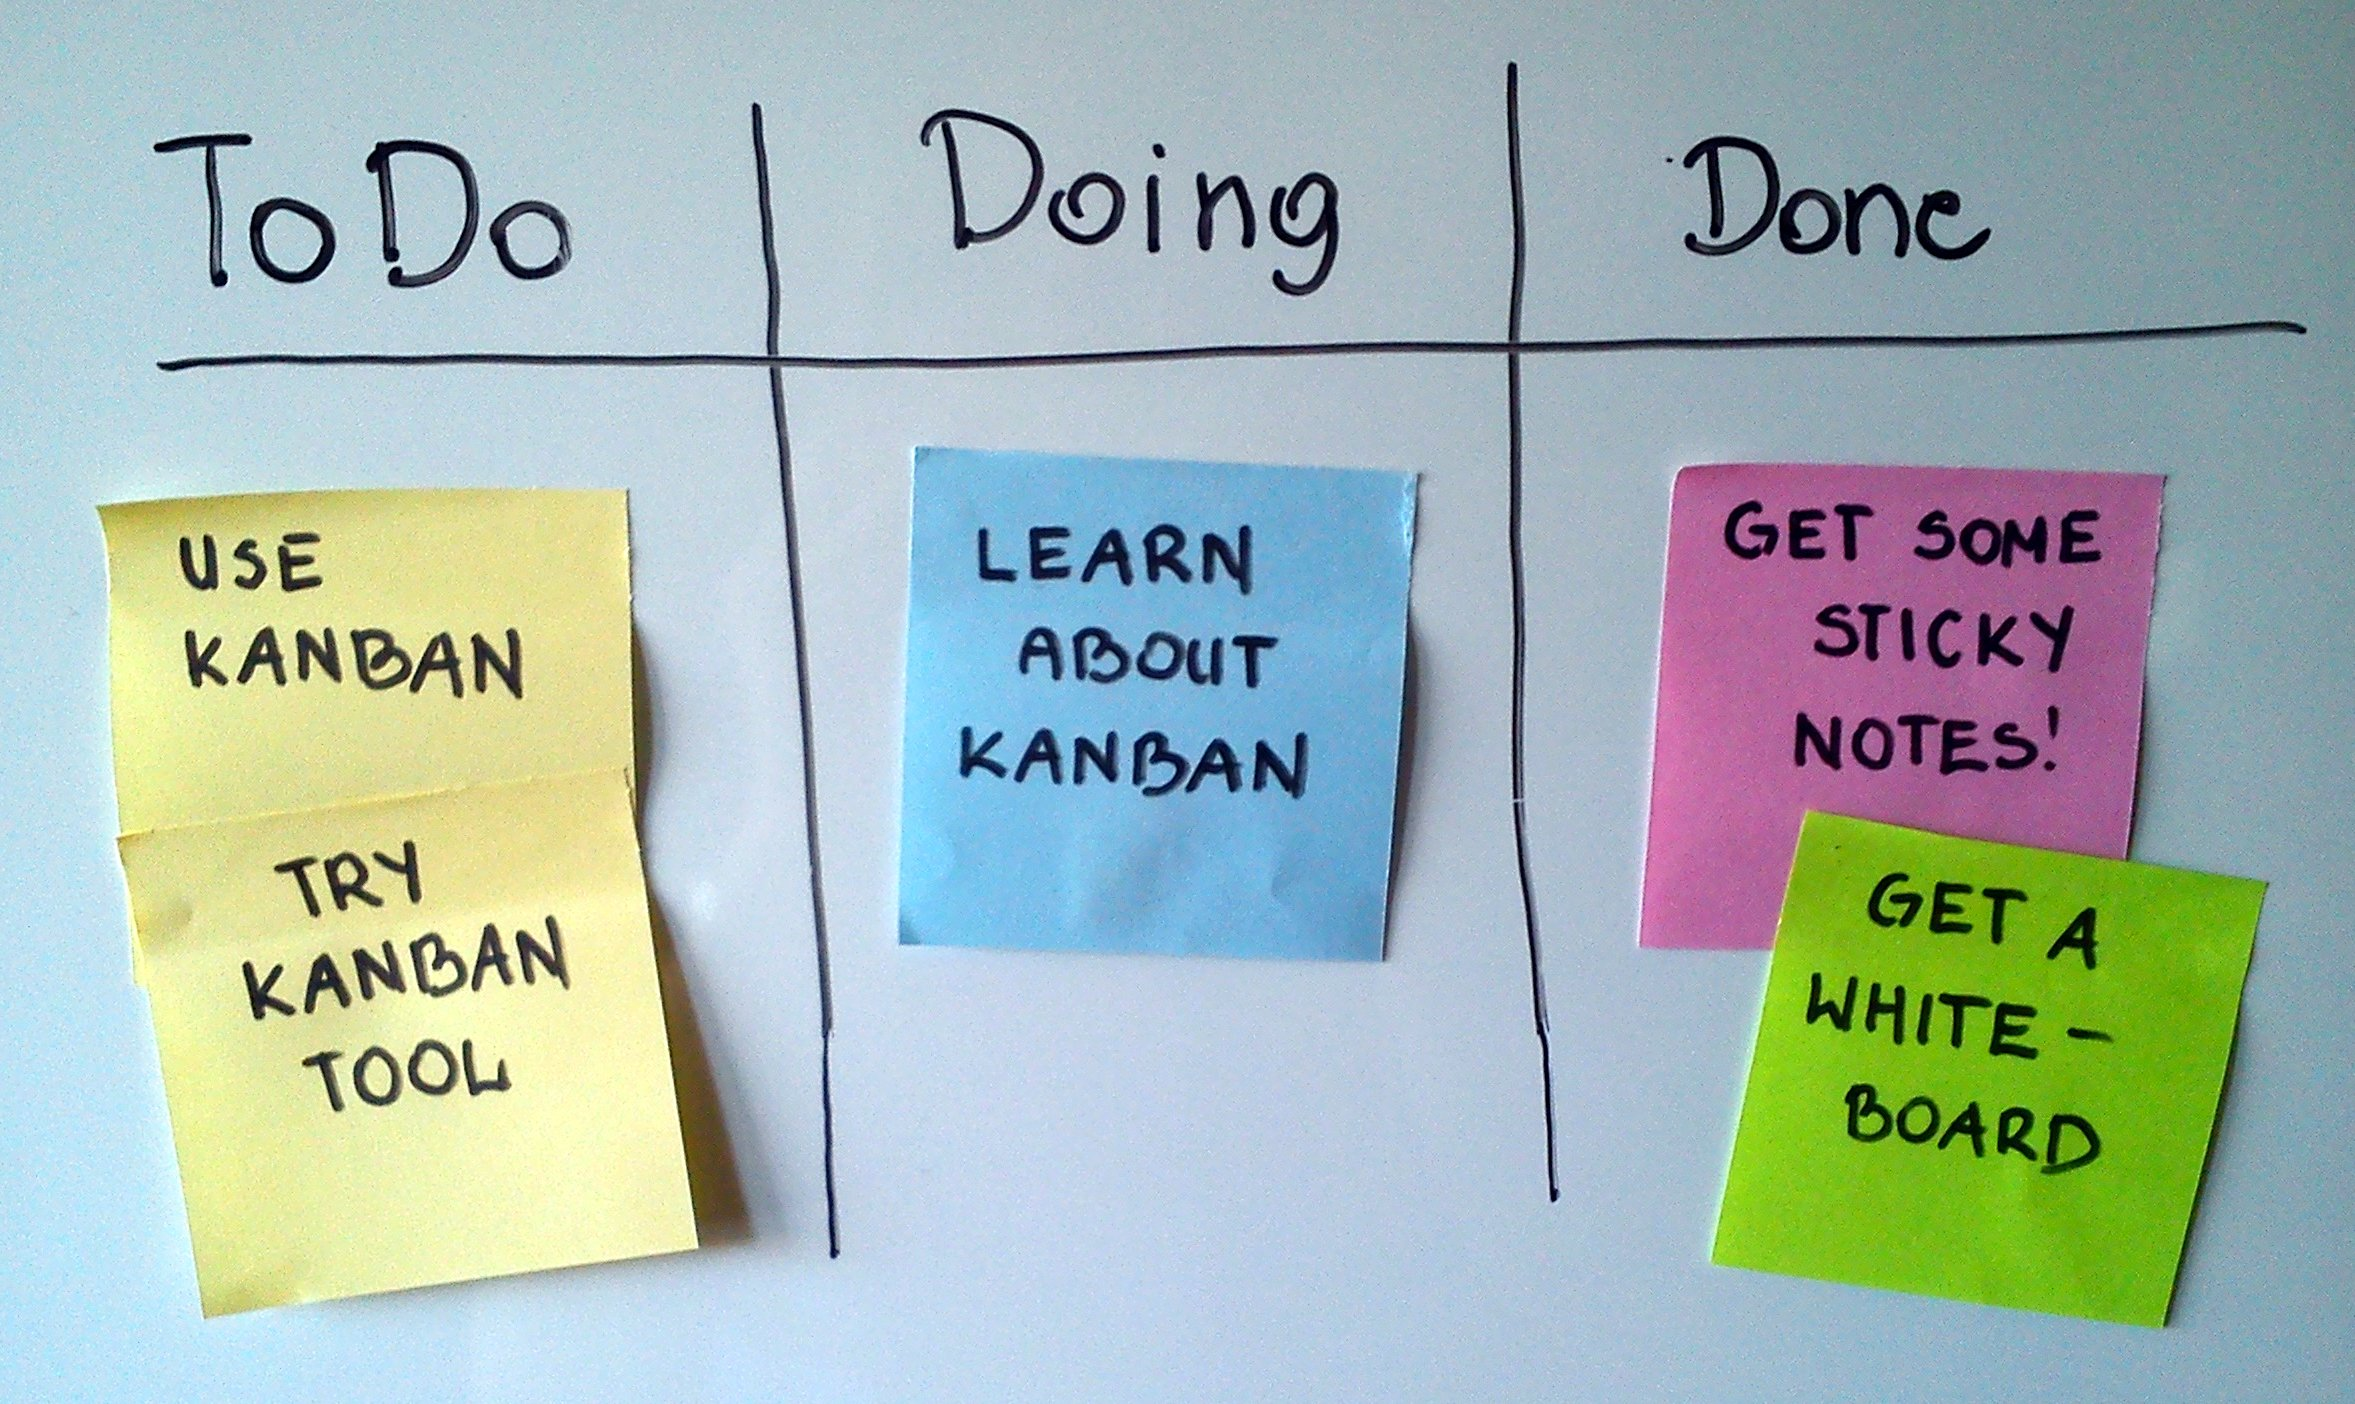
\includegraphics[width=\othersize]{imagens/Simple-kanban-board-.jpg}
    \caption{Um quadro Scrum/Kanban muito simples. Fonte:  por Jess Iasovski, CC BY-SA 3.0 }
    \label{fig:kanban}
\end{figure}

\subsection{O \textit{Project Model Canvas}}

O \textit{Project Model Canvas}\citep{finocchio:2013}, apresentado na Figura \ref{fig:pmcp}, é um canvas destinado ao planejamento inicial de um projeto, baseado em uma metodologia de 4 grandes passos, descrita na Figura \ref{fig:pmcp}. Ele possui 12 quadros que são preenchidas passo a passo na etapa de Concepção,  aprimorados nas fases de Integração e Revisão, e depois tem seu resultado comunicado as partes interessadas na fase de Compartilhamento. Sendo destinado a qualquer tipo de projeto, pode ser também aplicado a projetos de software, porém não necessariamente de forma perfeita.

\begin{figure}
    \centering
    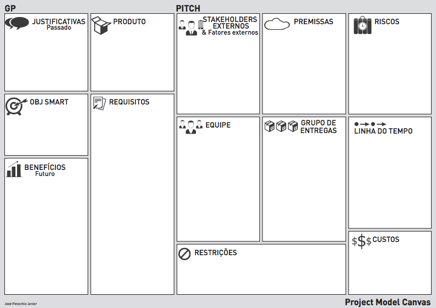
\includegraphics[width=\othersize]{imagens/ProjectMdoel Canvas.png}
    \caption{O processo de planejamento usando o Project Model Canvas. Fonte: \citet{finocchio:2013}}
    \label{fig:pmcp}
\end{figure}

Esse canvas é uma abordagem típica de projetos ágeis ou enxutos, aplicada ao planejamento de projetos de qualquer tipo. Isso é, simultaneamente, uma vantagem e uma desvantagem do \textit{Project Model Canvas}, já que, sendo geral, pode ser aplicado com sucesso em qualquer área, mas não sendo específico, acaba por ter algumas incompatibilidades com projetos de áreas específicas, como, e em especial, a Engenharia de Software.

Projetos de software têm características diferentes de projetos tradicionais que afetam diretamente o planejamento. Entre elas, podemos citar: a dificuldade de medir ou prever o tamanho da entrega, medido em esforço ou em prazo\citeauthor{mike:agile:estimating,cocomo2:manual,pressman:2019}, a necessidade de aprendizado da equipe em relação ao domínio da aplicação ao longo do projeto, a má-adequação às formas tradicionais e hierárquicas de equipe\citep{Constantine1993}. Essas e outras características que diferenciam o projeto de desenvolvimento de software afetam diretamente a capacidade de planejamento, exigindo estratégias diferenciadas em relação as estratégias tradicionais.

Ao ensinar e usar o \textit{Project Model Canvas} para o planejamento de projetos de desenvolvimento de software, notei algumas dificuldades dos alunos e praticantes com os quadros, listadas a seguir.

\begin{enumerate}
    \item A dificuldade de separar o pitch do produto e do objetivo SMART, e depois separar este do produto. Essas duas primeiras dificuldades advêm do fato de ser realmente difícil diferenciar o produto específico sendo criado do objetivo para o qual é criado. Isso, porém, pode não ser necessário no projeto de software, já que justificativas, benefícios e requisitos cumprem bem esse papel.
    \item A limitação a apenas um objetivo SMART para o software, quando é comum softwares atenderem várias funcionalidades que são normalmente criadas para atender objetivos;
    \item A dificuldade de separar requisitos não-funcionais de restrições;
    \item A não separação dos requisitos entre funcionais e não funcionais, tradicional na área de software, e importante no projeto de software, o que afeta diretamente a capacidade de estimar os custos do software, já que a prática mais frequente, formalizada nos Pontos de Função\citep{ifpug:guide:2012} e no COCOMO II\citeauthor{cocomo2:manual}, implica em calcular a funcionalidede entregue e depois melhorar a estimativa a partir de exigências feitas pelos requisitos não funcionais.
    \item Um excesso de esforço na separação entre grupos de entregas e linha do tempo, que ainda muitas vezes obriga a re-arranjar entregas ou requisitos, quando as práticas mais atuais, por exemplo baseadas em \textit{road-maps} do produto, tomam essa decisão de forma simultânea.
    \item \label{problems:total} A dificuldade de procurar custos, já que basicamente todo custo de um projeto de software vem da mão de obra, ou seja, do esforço necessário para desenvolve-lo, geralmente medido em pessoas-mês ou pessoas-hora.
\end{enumerate}

Todos esses problemas levam a uma ineficiência no processo de ensino e de uso do \textit{Project Model Canvas}, já que o tempo é gasto, repetidas vezes, na elucidação de conceitos ou restrições que não são essenciais ao projeto de software.

Para resolver essas dificuldades, este artigo propõe o uso do \textit{Software Project Canvas}. Além de ser criado especificamente para projetos de software, ele trata os problemas detectados no \textit{Project Model Canvas} da seguinte forma:
\begin{itemize}
    \item elimina o Pitch, substituindo-o pelo produto de software a ser criado;
    \item não apresente o objetivo SMART único, considerando que o objetivo é entregar o software;
    \item trata objetivos e metas com uma abordagem aceita na Engenharia de Software\citep{ruble_practical_1997};
    \item unifica no processo o tratamento de restrições e requisitos não-funcionais, para facilitar o processo de trabalho;
    \item separa os requisitos funcionais e não funcionais, os últimos com adição das restrições, em áreas diferentes do canvas, atendendo a prática comum da Engenharia de Software \citep{pressman:2019};
    \item unifica entregas e linha do tempo em uma caixa, onde as entregas já devem vir com uma data, ou será criado um roadmap do produto, típica de gestão ágil, e
    \item transforma todo o cálculo do custo em uma previsão do esforço\citep{mike:agile:estimating}.
\end{itemize}

Como resultado, o processo é transformado de 12 para 9 passos, já que mesmo em áreas separadas no canvas os requisitos são todos levantados no mesmo momento, facilitando sua explicação. Além disso, são evitadas muitas discussões desnecessárias, como onde colocar algo que tanto pode ser visto como uma restrição ou como um requisito não-funcional, por diferentes partes interessadas.

\section{O \textit{Software Project Canvas}}

O Software Project Canvas utiliza 10 quadros, que serão descritos nesta seção. Para cada quadro foi buscado explicar o que ele trata, métodos que podem ser usados para auxiliar seu preenchimento e alguns exemplos. Os quadros se organizam em 6 grupos que respondem às perguntas 5W2H\citep{nakagawa:2012:5w2h}: \textit{Why, What, Who, When, How} e \textit{How Much}. Não é necessário, em geral, reponder a pergunta \textit{Where}.

\begin{itemize}
    \item Por que: o que justifica o projeto, os Problemas e Oportunidades, e os Objetivos e Metas;
    \item O que: o que é o projeto, indicado pelos Requisitos Funcionais, Requisitos Não-Funcionais e Restrições;
    \item Quem: indicado pelas Partes Interessadas e a Equipe;
    \item Como: indicado pelos Subsídios e Premissas;
    \item Quando: indicado pelas Entregas, e
    \item Quanto: indicado pelos Riscos e Esforço.
\end{itemize}

\subsection{Problemas e Oportunidades}

Todo projeto se inicia porque há algum problema a ser resolvido ou uma oportunidade a ser aproveitada. Ou seja, se deseja uma mudança no estado da organização. Nas discussões sobre projetos de software, os problemas logo aparecem na forma de descontentamento com um sistema atual que funciona com falhas, erros ou não-conformidades.

Um problema é uma diferença entre um estado percebido e um estado desejado que deverá ser tratada pelo projeto. São dificuldades a serem resolvidas, desvios de um padrão, regulamento ou lei, falta de capacidade de realizar uma tarefa, etc. 

Problemas trazem prejuízo, sejam eles financeiros ou de outra forma, como impacto na imagem da empresa. Quando esses prejuízos podem ser medidos, deve ser indicada a forma de medi-los, de maneira que isso possa ser usado para verificar os benefícios que o projeto trará.

Os problemas podem ser divididos de várias formas. Uma delas é entender que existem problemas por não fazer algo, problemas funcionais, ou por não fazer algo como deve ser feito, problemas operacionais. Ambos tem efeitos no negócio, que são problemas de negócio, ou sintomas. Um problema de negócio pode ser a existência de longas filas em um restaurante, que pode ser causado por um problema operacional, a demora no cálculo da conta. Outro problema de negócio pode ser a dificuldade de entrar em contato com os clientes, que pode ser causado por um problema funcional, como a não existência de um cadastro de clientes.

Problemas podem ser descobertos e priorizados com uso de método de Pareto. É possível, porém, que o método de Pareto detecte apenas os sintomas. Por exemplo, se usarmos o método de Pareto para analisar as reclamações feitas em um restaurante, podemos descobrir que a maioria é sobre o excesso de tempo de espera na fila. Porém, esse não é o verdadeiro problema, mas sim um sintoma causado por, entre outras coisas, a demora em fechar uma conta. Para identificar as causas-raiz dos problemas, ou seja, o verdadeiro problema que deve ser resolvido, podem ser usadas técnicas como o Diagrama de Espinha de Peixe, ou os 5 Porquês\citep{gray:2010}. Existem outras técnicas disponíveis, principalmente na literatura de Controle de Qualidade em geral ou Qualidade de Software.

Já as oportunidades são percepções que algo pode ser feito para que a organização tenha uma vantagem em relação ao estado atual. Oportunidades podem ser levantadas de várias formas, incluindo o uso de \textit{brainstorming}\citep{tracy:2015}. 

Problemas e oportunidades podem ser priorizados por meio de técnicas como MoSCoW\citep{dsdm:2nd} e dot-voting\citep{gray:2010}.

Exemplos de problemas: documentos perdidos, perda de vendas ao longo do processo, fila excessiva, reclamações dos clientes, reclamações dos fornecedores.

Exemplos de oportunidades: novo produto vai ser lançado, dados disponíveis para data mining.

\subsection{Objetivos e Metas}

Nesta seção do \textit{Software Project Canvas} serão apresentadas as melhorias que o sistema traz ao negócio. A certa confusão dos termos objetivos e metas, então faremos uma definição desses termos para o \textit{Software Project Canvas}. Outro termo que pode ser usado é benefício.

Objetivos são mudanças que desejamos na organização. Esses objetivos devem ser SMART, isto é: e\textbf{S}pecíficos, \textbf{M}ensuráveis, \textbf{A}lcançáveis, \textbf{R}ealistas ou \textbf{R}ealizáveis, e delimitados no \textbf{T}empo. Por exemplo, construir um muro (S), de 2 metros de altura (M), com tijolos (A), a um preço de R\$2000,00 (R), em um mês(T).

Metas são resultados que esperamos quando houver a mudança trazida pelo projeto, ou seja, os benefícios trazidos ao negócio por termos alcançados os objetivos. Metas precisam de medidas, subjetivas ou objetivas, também chamadas de qualitativas ou quantitativas, associadas a elas. Por exemplo, o muro pode ter sido colocado para diminuir a quantidade de pessoas que entra em um local, o que pode ser contado, ou para aumentar a sensação de segurança dos moradores, o que é um sentimento subjetivo. Cada objetivo deve ter pelo menos uma meta, e cada meta uma forma de avaliar\cite{ruble_practical_1997}. 
Todo objetivo, e suas metas, deve endereçar um item que aparece na justificativa\cite{finocchio:2013}.

Uma das várias formas de buscar benefícios é usar a heurística IRACIS\footnote{Increase Revenue, Avoid Costs and Improve Service}, que os divide em 3 tipos: aumentar receitas, evitar cursos e melhorar serviços.

Exemplo de objetivo: detecção de necessidade de repor o estoque, com a meta diminuir reclamações e a métrica número de reclamações que um item não estava no estoque, ou número de vendas perdidas porque o item não estava no estoque.

\subsection{Requisitos Funcionais, Não-Funcionais e Restrições}

Segundo a norma ISO/IEC/IEEE 24765:2017, `` um requisito é uma condição ou capacidade necessária para uma parte interessada resolver um problema ou atingir um objetivo.'', ou, ainda segundo a mesma norma, ``Ele deve ser possuído ou alcançado por um sistema, componente de um sistema para satisfazer um contrato, padrão, especificação ou outro documento formalmente imposto''\citep{IEEE:24765:2017}.

Requisitos podem ser divididos em dois grandes grupos: funcionais ou não-funcionais. Restrições são tipos especiais de requisitos funcionais impostos ao projeto. Requisitos funcionais dizem que funcionalidade o software entrega, na prática, que funcionalidades o usuário exige do software. Já requisitos não-funcionais especificam como essas funcionalidades devem acontecer ou desempenhar. Requisitos funcionais são, em geral, independentes de tecnologias.

Os Requisitos Não-Funcionais, Restrições e Requisitos Funcionais podem ser levantados no mesmo passo, apesar de haver uma separação no quadro. Isso facilita a discussão do que deve ser entregue, pois não é necessário dizer ``guarde esse requisito para o próximo passo''. 

\subsubsection{Requisitos Funcionais}

Requisitos funcionais dizem o que o software deve fazer. Recomendamos que isso seja feito na forma de histórias do usuário, cujo formato padrão é uma frase do tipo ``Como gerente, eu quero listar os vendedores e suas vendas, para determinar os melhores vendedores da empresa''\citep{mike:user:stories}.

Outra forma possível é usar objetivos do usuário, ou seja, os nomes de casos de uso, como: listar melhores vendedores\citep{Cockburn2000}.

É importante usar uma estratégia para não deixar a lista de requisitos funcionais muito longa. A primeira é usar casos de uso ou história de usuário de nível de abstração alto, ou seja, usar uma estratégia \textit{top-down} no desenvolvimento dessa lista. Dessa forma, os requisitos poderiam ser semelhantes aos encontrados em uma história do usuário de alto nível\citep{jacobson:2011:uc2p0}, em uma DFD de nível 0\citep{gane:sarson:ssa}, ou ainda em diagrama de casos de uso do nível pipa ou nuvem\citep{Cockburn2000}. O outro é listar apenas os mais importantes. Para isso, pode ser usada a técnica de priorização MoSCoW\citep{babok,dsdm:2nd} para eliminar os requisitos não adequados a fase inicial.

Exemplos de requisito funcional são:
\begin{itemize}
    \item no caso de usar casos de uso: comprar livros, enviar mensagem, relatar ausência de item no estoque, e
    \item no caso de histórias do usuário: como gerente eu quero listar os vendedores e suas vendas para descobrir os melhores vendedores, como leitor eu quero listar os novos lançamentos para poder decidir que livro vou comprar.
\end{itemize}

\subsubsection{Requisitos Não-Funcionais e Restrições}

Requisitos não-funcionais e restrições falam da forma como os requisitos funcionais vão ser alcançados. Apesar de podermos considerar que os requisitos não-funcionais são desejados e as restrições são impostas, é difícil para um pessoa não-treinada fazer essa separação de forma rápida, então não nos preocupamos em fazê-la agora. Em outra fase do processo de criação do \textit{Software Project Canvas}, as restrições, ou requisitos não-funcionais, que inviabilizam o trabalho, podem ser eliminadas ou amenizadas.

Podem ser de vários tipos e conhecer uma taxonomia pode ajudar a levantá-los. \citet{sommerville:software:2015} apresenta uma hierarquia de requisitos não funcionais que foi adaptada na Figura.

\begin{figure}
    \centering
    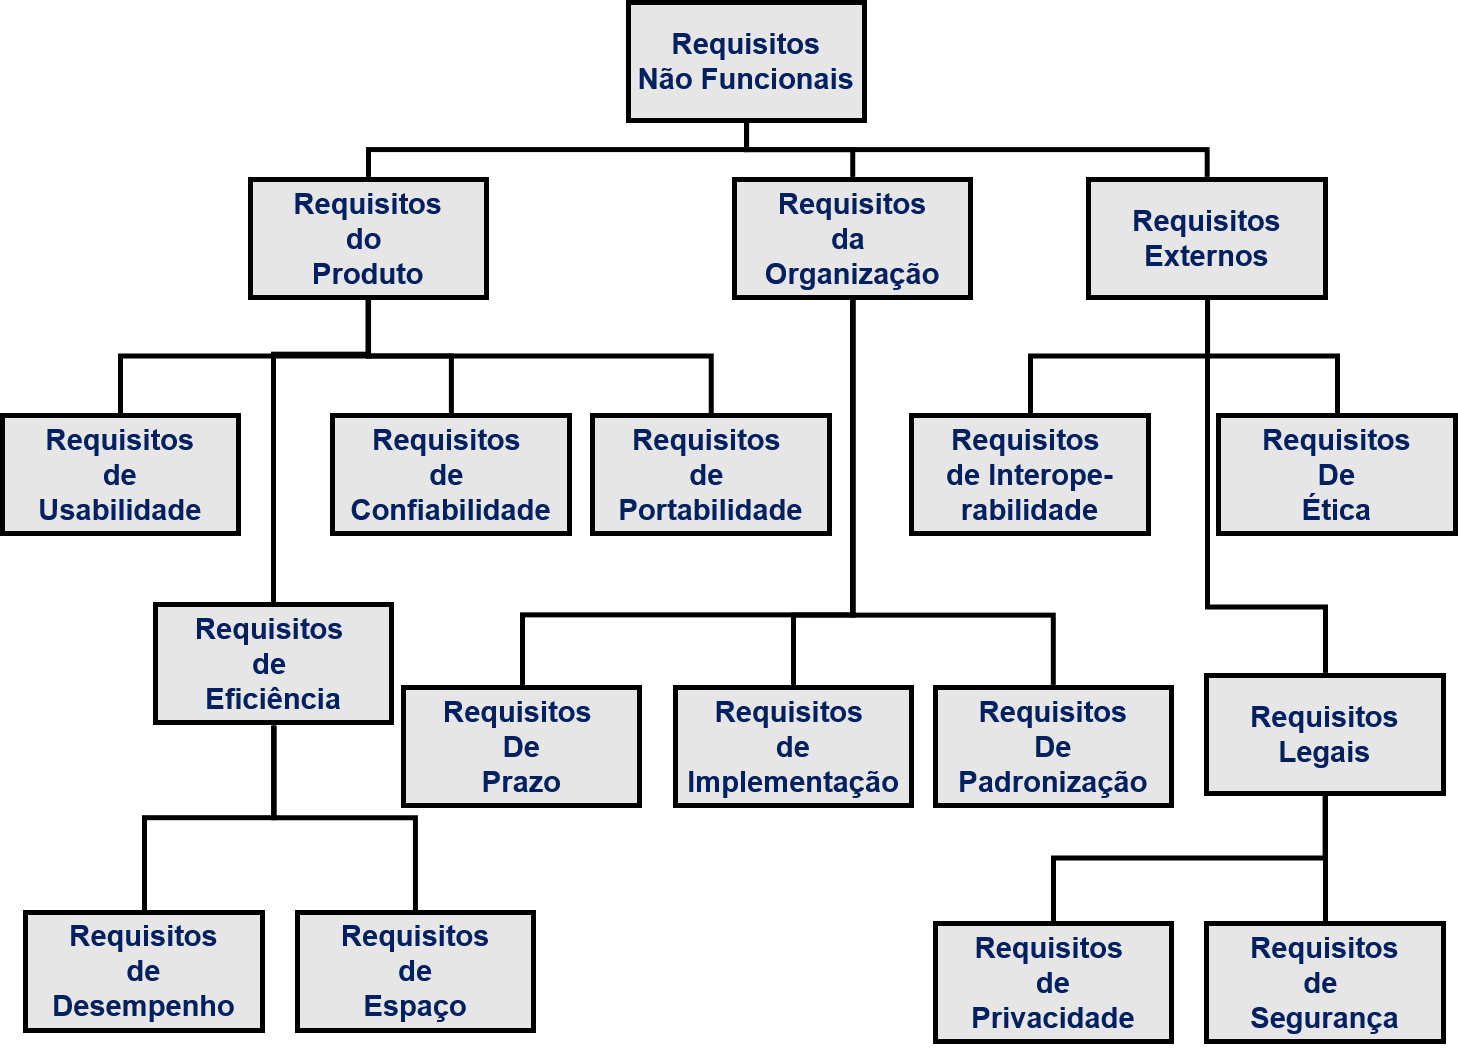
\includegraphics[width=\othersize]{imagens/NonFunReq.png}
    \caption{Taxonomia de Requisitos Não Funcionais. Fonte: \citet{sommerville:software:2015}}
    \label{fig:nofunreq}
\end{figure}

Restrições limitam o trabalho realizado e devem ser bem específicas, quantificadas e ainda indicar por quem são impostas.

Os requisitos não-funcionais podem ser associados a todos ou apenas a alguns requisitos funcionais. Se for o caso, é interessante fazer essa indicação.

Exemplo de requisito não-funcional: mensagens devem ser na forma de e-mail, o envio de um e-mail deve demorar no máximo 2 minutos, a senha deve seguir as regras de segurança definidas pela empresa. Exemplos de restrições: a linguagem de programação só pode ser Java, o banco de dados usado pelo projeto tem que ser Oracle 10.

\subsection{Partes Interessadas}

Uma parte interessada (P.I.), ou \textit{stakeholders}, é um indivíduo, grupo ou organização que pode afetar, ser afetado, ou perceber que será afetado, por uma decisão, atividade, ou resultado, parcial ou final de um projeto\citep{pmbok:6}.

As partes interessadas  podem ter opiniões diferentes em relação ao projeto, seja por sua participação ou interesse, quanto a percepções, corretas ou incorretas, que o resultado final ou parcial, vai afetá-la positiva ou negativamente.  Algumas serão consideradas \textit{champions} do projeto, outras podem ser neutras, e ainda outras abertamente, ou secretamente, contra o projeto.

Identificar as todas as partes interessadas é o passo inicial dos processos de gestão das partes interessadas\citep{jacobson_essentials_2019,pmbok:6}, com o objetivo de garantir a satisfação das mesmas, e com isso o sucesso do projeto. No SEMAT, por exemplo, identificar as partes interessadas é o primeiro estado para o Alpha \textit{Stakeholders}, seguido da escolha de representantes\citep{jacobson_essentials_2019}.  Os estados seguintes são: envolvidas, em acordo, satisfeita para a implantação e satisfeita com o uso\citep{jacobson_essentials_2019}.

Nessa parte do \textit{Software Project Canvas} são listadas todas as partes interessadas  do projeto. Devem ser consideradas especialmente três tipos de P.I., os usuários finais, o patrocinador e o governo, como órgão legislador a que o projeto pode estar submetido. Para listá-las, pode ser necessário o uso de técnicas como \textit{brainstorming}\citep{tracy:2015} ou \textit{writestorming}\citep{gray:2010}.

Outras partes interessadas comuns de encontrarmos: clientes dos usuários, fornecedores dos usuários, futuros operadores do software, sistemas que podem ser acessados ou acessar o software, e seus mantenedores, organizações e suas partes que podem ter algum interesse no resultado do software.

É importante que sejam usadas, sempre que possível, termos ligado ao negócio. Assim, um médico não tem clientes, mas pacientes, enquanto um banco tem correntistas.

Fatores externos fora do controle do projeto também podem ser listados aqui. Não é incomum que projetos de software sofram o impacto do valor do dólar, por exemplo.

Por conveniência do processo de definição do projeto de software, a equipe de desenvolvimento, que é, em geral, uma parte interessada, não deve ser considerada nesse momento.

Exemplos de partes interessadas são: vendedores, compradores, pacientes, patrocinador, diretoria de operações, etc.

\subsection{Equipe}

Nesse quadro é indicada a equipe necessária para o desenvolvimento do projeto. Cada \textit{post-it} deve indicar um papel a ser tomado pelos membros da equipe. Quando for necessário mais de uma pessoa, isso deve ser indicado no mesmo \textit{post-it}. Possivelmente, algumas pessoas podem estar nomeadas no mesmo \textit{post-it}, ou em outro, de outra cor, possivelmente menor, colocado sobre o primeiro.

Alguns papéis são esperados\citeauthor{finocchio:2013}, como o gerente do projeto e um ou mais programadores. Alguns papéis também são esperados em funções do processo de desenvolvimento de software sendo usado. Por exemplo, se é usado o Scrum, esperamos encontrar o Scrum Master, o Product Owner, que pode, por outro lado, ser listado como parte interessada, e o Time, que será formado de várias pessoas.
\subsection{Subsídios e Premissas}
Nesta seção do \textit{Software Project Canvas} devem aparecer tudo necessário para que o projeto tenha sucesso. Tipicamente, em projetos de software, subsídios e premissas estão ligados ao acesso da equipe as P.I., e a participação das mesmas quando necessário. Também é comum que existam premissas ligadas a disponibilidade da infraestrutura necessária para o sucesso do projeto. Em muitos projetos também é necessário tratar aqui a disponibilidade financeira.

Premissas e subsídios são garantidas pelas partes interessadas, em favor da equipe. Caso uma parte interessada não cumpra seu compromisso em garantir a premissa, ocorre um risco do projeto. Assim, a análise de risco deve considerar todas as premissas feitas. 

Exemplo de premissas ou subsídios: os computadores novos serão entregues dia 15 de maio, os computadores possuirão uma placa gráfica compatível com a NVidia 3060, serão contratados cinco novos programadores, o patrocinador disponibilizará 4 horas por semana para o projeto. 

\subsection{Entregas}

Um projeto de software moderno é feito de forma iterativa e incremental\citep{pressman:2019,essential:scrum}, o que implica em várias pequenas entregas, que se iniciam com protótipos, provas de conceito ou um produto mínimo viável, e se seguem de versões ou \textit{releases} que fornecem cada vez mais valor aos seus usuários.

Essas entregas devem ser previstas, sendo que as entregas a curto prazo devem ser prevista com mais detalhe de que as de longo prazo, já que os métodos de desenvolvimento de software se tornaram, na sua maior parte, adaptativos.

Em cada entrega é entregue um conjunto de funcionalidades, ou seja, são cumpridos requisitos funcionais. Também são garantidos os requisitos não funcionais e as restrições. Assim, as entregas devem ser construídas a partir desses quadros anteriores, levando em consideração a equipe prevista.

É possível que as entregas sejam descritas de forma a implementar parcialmente vários requisitos de forma parcial, como o que é proposto em \citetitle{jacobson:2011:uc2p0}\citep{jacobson:2011:uc2p0}. Por exemplo, um requisito que diga ``Como professor eu quero enviar mensagens para alunos para dar avisos sobre a próxima aula'', pode em uma entrega enviar e-mails, na seguinte incluir mensagens por WhatsApp, e assim por diante. Nesse caso, deve haver cuidado na descrição das entregas, para deixar claro que os requisitos não são cumpridos integralmente.

Entregas também podem ser desenvolvidas, mais tarde, ou como resultado intermediário para gerar o \textit{Software Project Canvas}, por meio de uma Estrutura Analítica de Projeto (EAP), também conhecida pelo nome em inglês, que faz mais sentido, \textit{Work Breakdown Structure (WBS)}. Nesse caso, deve ser seguida a abordagem de criar uma hierarquia de entregas, e não de processos.

Exemplos de entregas: lista de livros, seleção e compra - em 40 dias; relatórios de acompanhamento - em mais 20 dias, sistema de recomendação - em 60 dias; 

\subsection{Riscos}

Riscos são incertezas que podem influenciar o resultado do projeto. Atualmente riscos são divididos em ameaças e oportunidades, isto é, existem riscos negativos e positivos.


É importante para a gestão do projeto gerenciar o risco, para isso devem ser conhecidos sua causa, isto é, porque ele acontece, sua probabilidade de ocorrer e seu impacto. Com isso é possível calcular o efeito do risco no projeto.

Os riscos podem ser aceitos desprezados, por terem um impacto baixo, aceitos e gerenciados, mitigados, ou, ainda, eliminados ou transferidos. Essas ações foram listadas do que deve ser feito para os riscos de impacto mais baixo até o mais alto. 

Todo projeto tem riscos gerais e específicos. Riscos gerais são geralmente reconhecidos pela comunidade. Um risco típico de projeto de software é a perda de um membro importante da equipe, ou que possui um conhecimento único.


Toda premissa é candidata a gerar um risco, que deverá ser analisado. Existem categorias reconhecidas, pode riscos técnicos, externos, organizacionais ou de gerenciamento\citep{pmbok:6}. 
Para os riscos gerais podemos encontrar \textit{checklists} que podem ser seguidas. Já para os riscos específicos é necessário analisar atentivamente o projeto, suas premissas, complexidades e outros fatores. 

Existem várias heurísticas para tratar o risco, mas a princípio, para cada risco levantado deve ser estimada sua probabilidade e seu impacto. O produto dos dois implica em uma reação. \citet{finocchio:2013} sugere usar duas escalas de 1 a 10 para avaliar a probabilidade e o impacto, fazendo o produto e obtendo as recomendações segundo a Tabela.

\begin{table}[hbt]
    \centering
    \begin{tabular}{cc}
    \toprule
     Probabilidade $\times$ Impacto    &  Ação  \\
     \midrule
         1 a 3  & Aceitar passivamente \\
         4 a 10 & Aceitar ativamente, com um plano de resposta \\
         11 a 36 & Mitigar o risco \\
         37 ou mais & Eliminar ou transferir o risco \\
    \bottomrule
    \end{tabular}
    \caption{Ações recomendadas por \citep{finocchio:2013} de acordo grau de importância do risco}.
    \label{tab:risco}
\end{table}

Exemplo de riscos: não conseguir contratar cinco novos funcionários com a habilidade necessária (probabilidade 7, efeito 8), servidor atual não aguentar a carga do novo sistema.

\subsection{Esforço}

Nesse quadro deve ser estimado o esforço para desenvolver o software em homens-mês ou homem hora. No momento da reunião onde o canvas é usado, não é possível ainda usar uma técnica fortemente quantitativa para isso, como o COCOMO II\citep{Boehm:cocomo2}, pois não se espera que seja possível nem estimar o tamanho real do software, então isso deve ser feito a partir da experiência do grupo, com comparações com projetos anteriores. 

Técnicas adequadas nesse ponto são variações do método de Delphi\citep{delphi:1966}, como o \textit{Planning Poker}\citep{mike:agile:estimating}, ou uso de heurísticas como buscar previsões pessimistas ($P$), médias ($M$) e otimistas ($O$) e calcular uma média ponderada ($M_p=\frac{P+4\times M+O}{6})$\citep{pmbok:6}.

\section{A Metodologia do \textit{Software Project Canvas}}

A metododologia utilizada do \textit{Software Project Canvas} possui 4 grandes passos, sendo inspirada na metodologia proposta pelo \textit{Project Model Canvas}. Ele está descrita em BPMN nas Figuras \ref{fig:bpmn1} e \ref{fig:bpmn2}

\begin{figure}[htb]
    \centering
    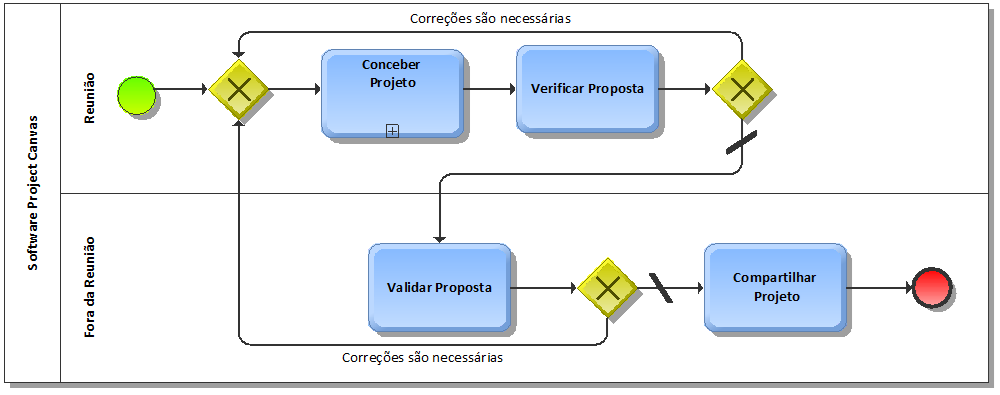
\includegraphics[width=\textwidth]{imagens/Software Project Canvas - 4 pessos.adf.png}
    \caption{Descrição do processo de criação do Software Project Canvas. Fonte: imagem do autor}
    \label{fig:bpmn1}
\end{figure}

\subsection{Conceber Projeto}

A principal atividade criativa da metodologia é Conceber o Projeto. Isso é feito em uma, ou mais, reuniões facilitadas, em que o Canvas é usado como foco de colaboração. Os passos dessa reunião são descritos na Figura \ref{fig:bpmn2}, porém esse segundo processo deve ser entendido de forma genérica, já que não há proibição de se voltar a um passo anterior para melhorar, apagar ou propor novos itens.

\begin{figure}[htb]
    \centering
    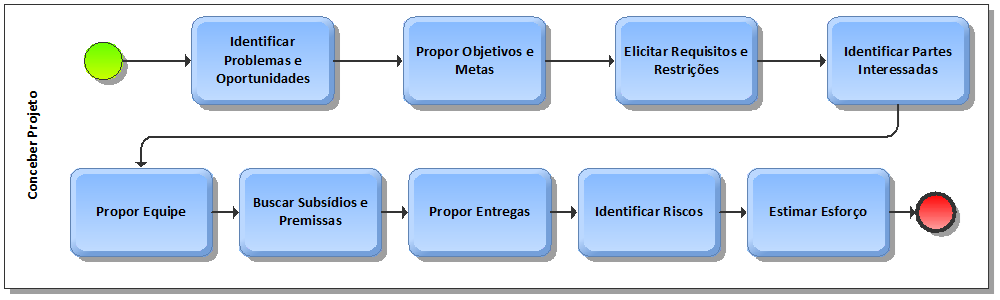
\includegraphics[width=\textwidth]{imagens/Conceber Projeto do Software Project Canvas.png}
    \caption{Descrição do sub-processo Conceber Projeto, do processo de criação do Software Project Canvas. Fonte: imagem do autor}
    \label{fig:bpmn2}
\end{figure}


Essas reuniões devem contar com representantes da equipe e das partes interessadas, incluindo o patrocinador, clientes, e membros do escritório de projetos ou assemelhados, se essa função existir na organização. É essencial que existam pessoas com a compreensão da gestão de projetos de desenvolvimento software para liderar a reunião, explicar conceitos e trazer sua experiência nas propostas e estimativas.

Durante a reunião, cada passo é focada em preencher um quadro, e para isso deve ser usada uma estratégia em diamante, onde em um primeiro momento deve ser usada uma prática de divergência, ou geração criativa de ideias, normalmente o \textit{brainstorming}\citep{tracy:2015} ou técnica derivada, ou assemelhada, e em um segundo momento uma técnica de convergência,  seja ela de a busca de consenso, priorização ou votação, como por exemplo MoSCoW\citep{dsdm:2nd} ou \textit{dot-voting}\citep{gray:2010}. 

Os quadros devem ser inicialmente preenchidos sem limites, já que é necessário estimular a criatividade durante o momento de divergência. Já durante o momento onde se faz a convergência eles devem ser agrupados em ideias semelhantes e postos em ordem de prioridade, urgência ou importância. Além disso, é necessário garantir que todos os \textit{post-its} estejam em um mesmo nível de abstração, se necessário agrupando vários em um só, ou separando um em vários. 
Em cada passo, então, são colocados, modificados e retirados \textit{post-its} no canvas, até que os participantes estejam satisfeitos.

É importante notar que a metodologia faz, em um só passo, todo o levantamento de requisitos funcionais, não-funcionais, e restrições. Isso foi decidido pelo fato de, ao usar outras metodologias, ser comum que um item desses tópicos seja proposto enquanto outro tópico é feito. Unificando esse momento, não é necessário parar para discutir questões de ordem da reunião.

É possível que durante um quadro, como por exemplo premissa, se descubra a necessidade de incluir um novo \textit{post-it} em um quadro anterior, por exemplo, uma nova parte interessada. Isso é totalmente permitido, não sendo necessário refazer todo o trabalho do quadro anterior, porém devemos verificar com atenção esse novo item no próximo passo.

Ao longo da Concepção, é importante que os participantes da reunião estejam atentos às regras que serão usadas na verificação, principalmente no momento de convergência, para garantir desde início a qualidade do quadro.

É possível também usar \textit{post-its} com cores e tamanhos diferentes para dar significados específicos. Por exemplo, podem ser usados \textit{post-its} vermelhos para chamar atenção de itens que foram colocados em um quadro após eles já terem sido resolvidos em uma primeira passagem.

\subsection{Concepção Iterativa e Incremental}

É possível realizar a concepção do processo de forma iterativa e incremental, mesmo que em apenas uma seção. Para isso, se inicia cada iteração com um problema ou oportunidade, normalmente o mais importante, e se passa por todos os quadros atendendo apenas aquele problema, e mais nenhum outro. Ao terminar a iteração, deve ser analisado se é razoável fazer outra iteração ou o projeto já está definido. 

Durante cada iteração pode ser necessário adaptar o resultado das iterações anteriores para atender os requisitos da nova iteração. Por isso é importante manter alguma memória ao final de cada iteração, por exemplo fotografando o quadro, ou o reproduzindo rapidamente em uma ferramenta digital, como Miro ou mesmo o Power Point.

Mesmo que a próxima iteração do projeto vá resolver apenas o primeiro problema, é interessante já começar com alguns problemas, e suas solução subsequente, determinados, levando a criação de um \textit{road-map} do produto. Técnica similar é feita no Scrum, onde é mantido o Product Backlog e escolhido apenas um Sprint Backlog para realizar a cada iteração\citep{scrum:sbok:guide}.

Se o quadro é mantido fixo na parede ao longo do projeto, pode ser revisado também a cada iteração.

\subsection{Ordens Alternativas de Preenchimento}

Apesar de ser comum planejar um projeto na ordem inicial Por que, O que e Quem, definindo o contexto para o qual as outras perguntas vão ser respondidas, é possível fazê-lo em outra ordem.

O Software Project Canvas não impõe, então, que seja usada apenas a ordem proposta, e ainda oferece canvas pré-prontos para duas ordens alternativas:
\begin{itemize}
    \item iniciar com as Partes Interessadas, encontrar os Problemas e Benefícios que elas tem e só depois projetar o que será o projeto, e
    \item iniciar com o porquê, descobrir as partes interessadas e então passar para os requisitos.
\end{itemize}

Essas ordens alternativas representam situações diferentes na vida real. 

Na nossa proposta inicial, apresentada na Figura \ref{fig:spc} supomos que a organização tem problemas ou oportunidades, e a partir daí o projeto é criado e, então, olhando esse quadro, são determinadas todas as partes interessadas. 

Na segunda proposta, primeiro foi identificado que algumas partes interessadas estão descontentes, ou precisam de algo. É provável que estas partes interessadas estejam inclusive presente na reunião, e começar por identificá-las pode ajudar a procurar os problemas e seguir com o projeto. 

Finalmente, na terceira proposta, imaginamos que os problemas foram identificados, e logo depois identificamos quem está envolvido com esses problemas.

\begin{figure}
    \centering
    \begin{subfigure}[b]{\textwidth}
    \centering
    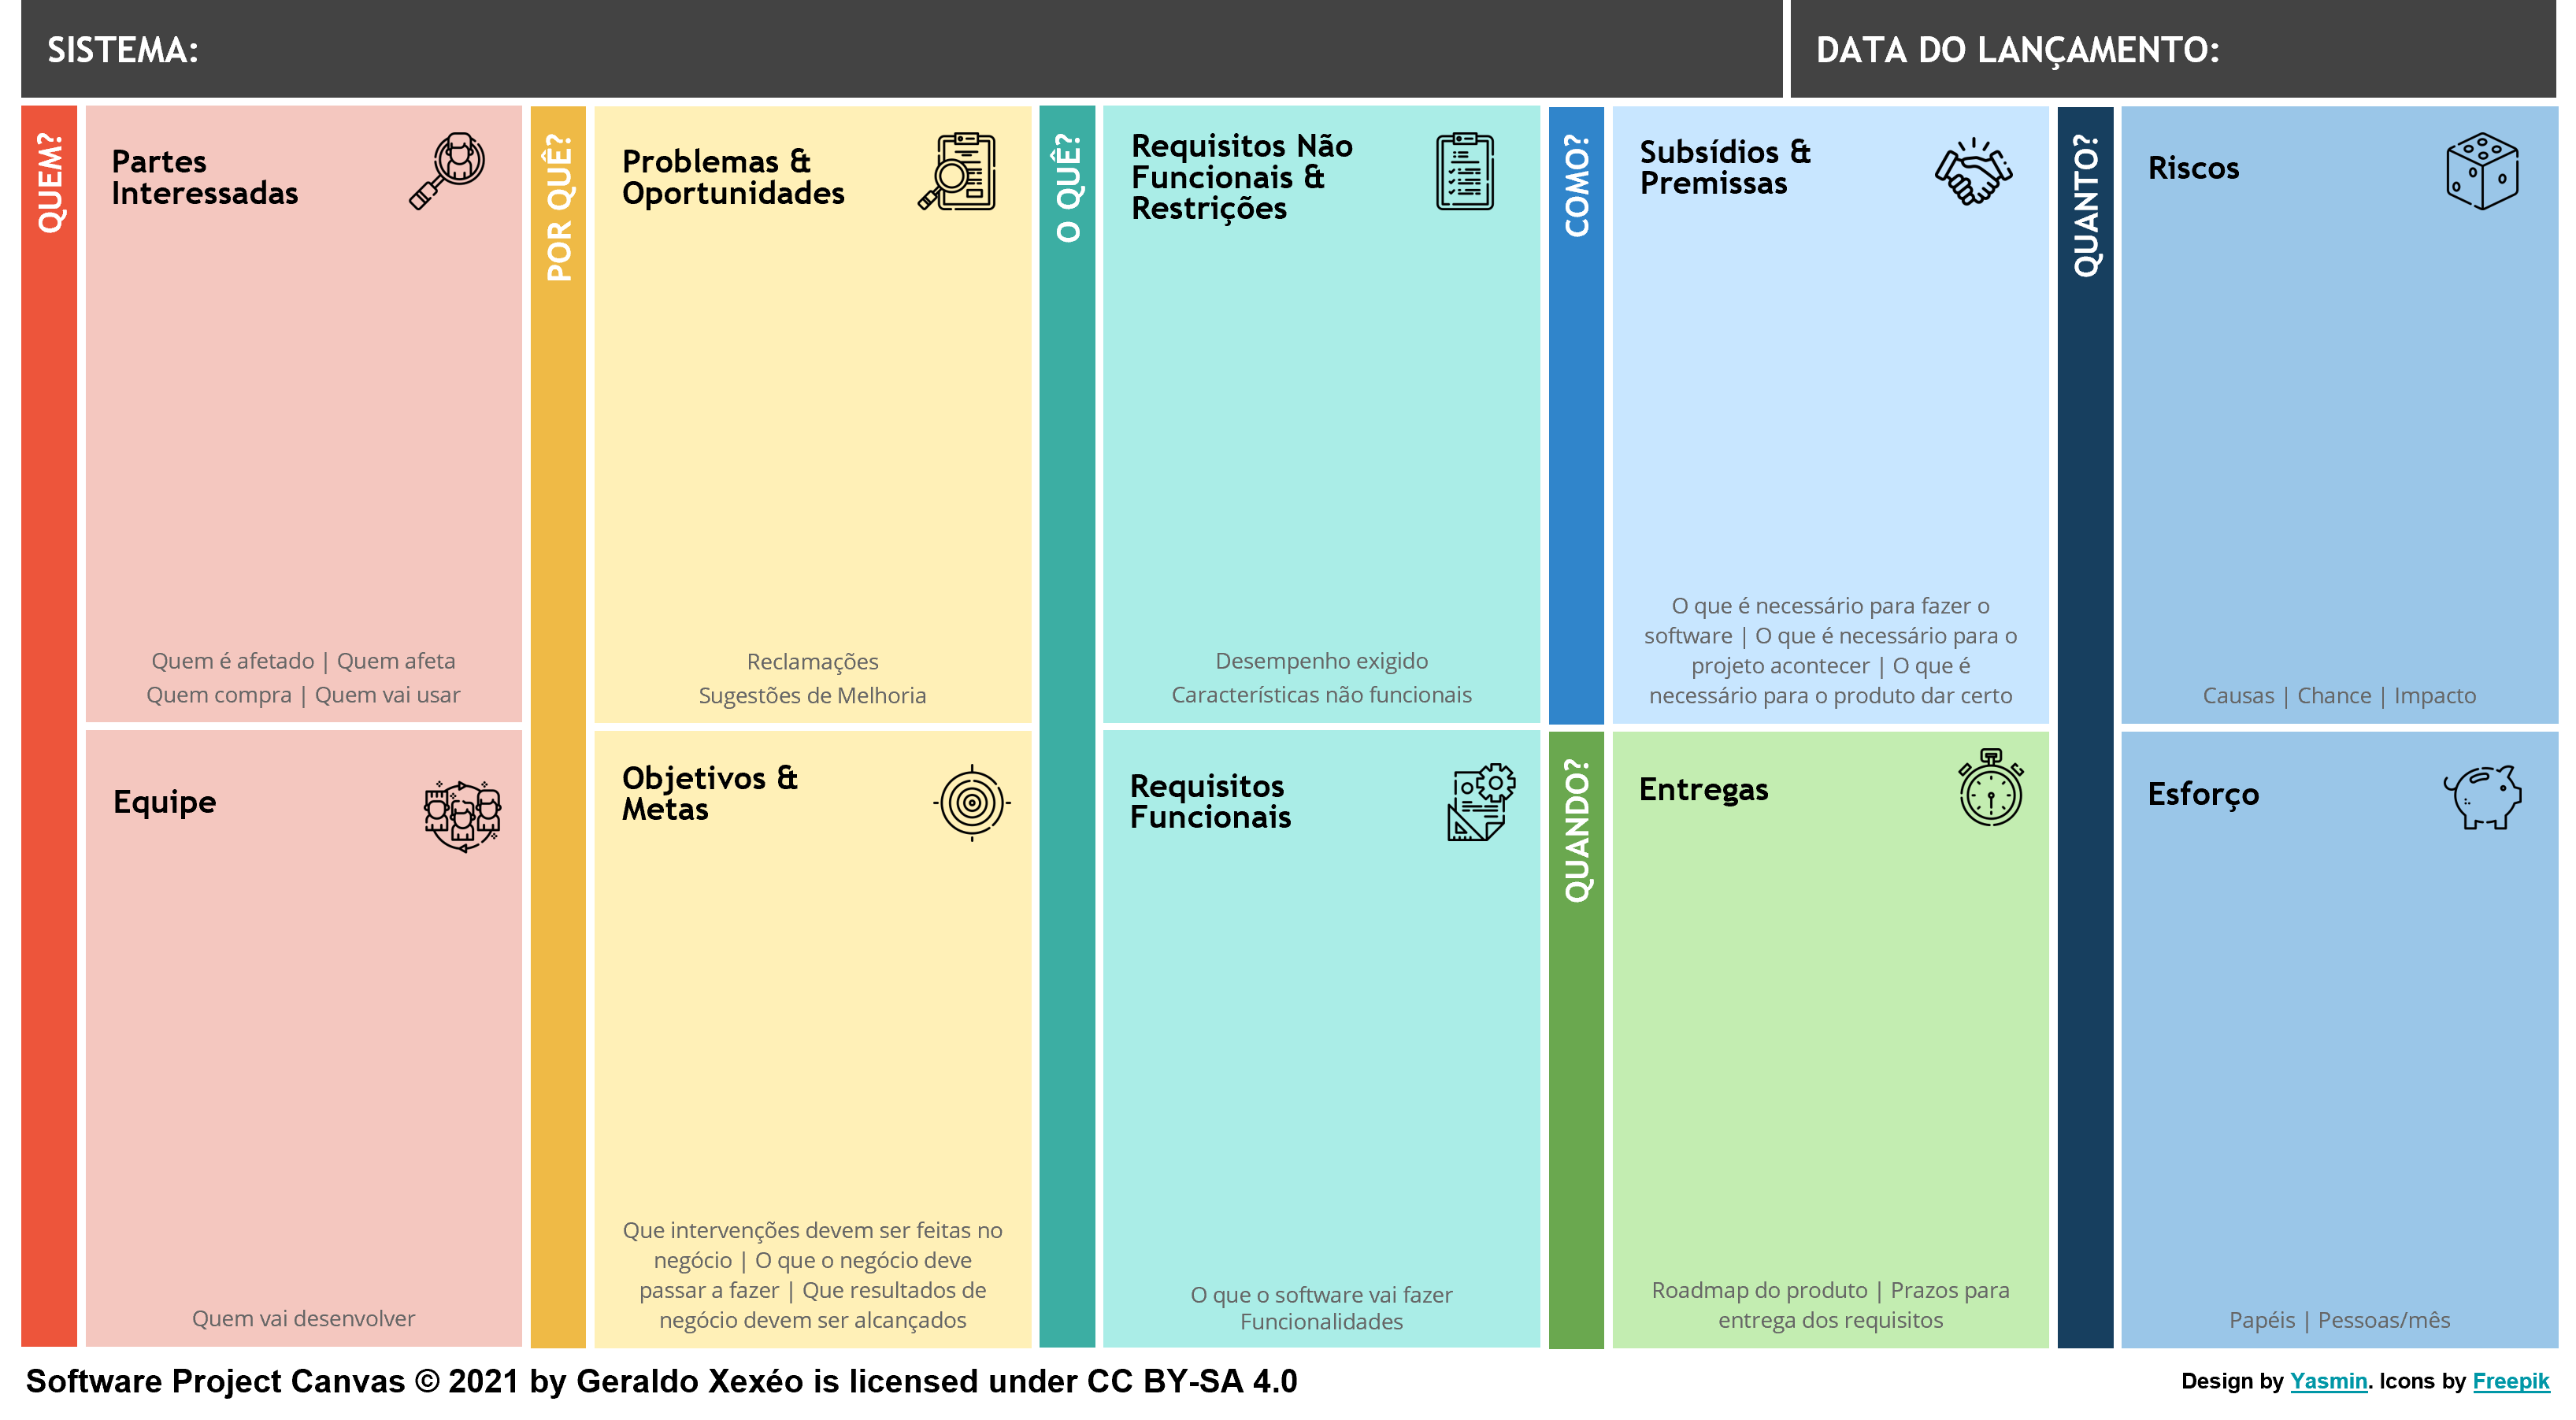
\includegraphics[width=0.9\textwidth]{imagens/alternativa2.png}
    \caption{Forma alternativa onde o projeto se inicia com as partes interessadas. Fonte: imagem do autor}
    \label{fig:alter2}
    \end{subfigure}
    
    \vspace{1cm}
    
    \begin{subfigure}[b]{\textwidth}
    \centering
    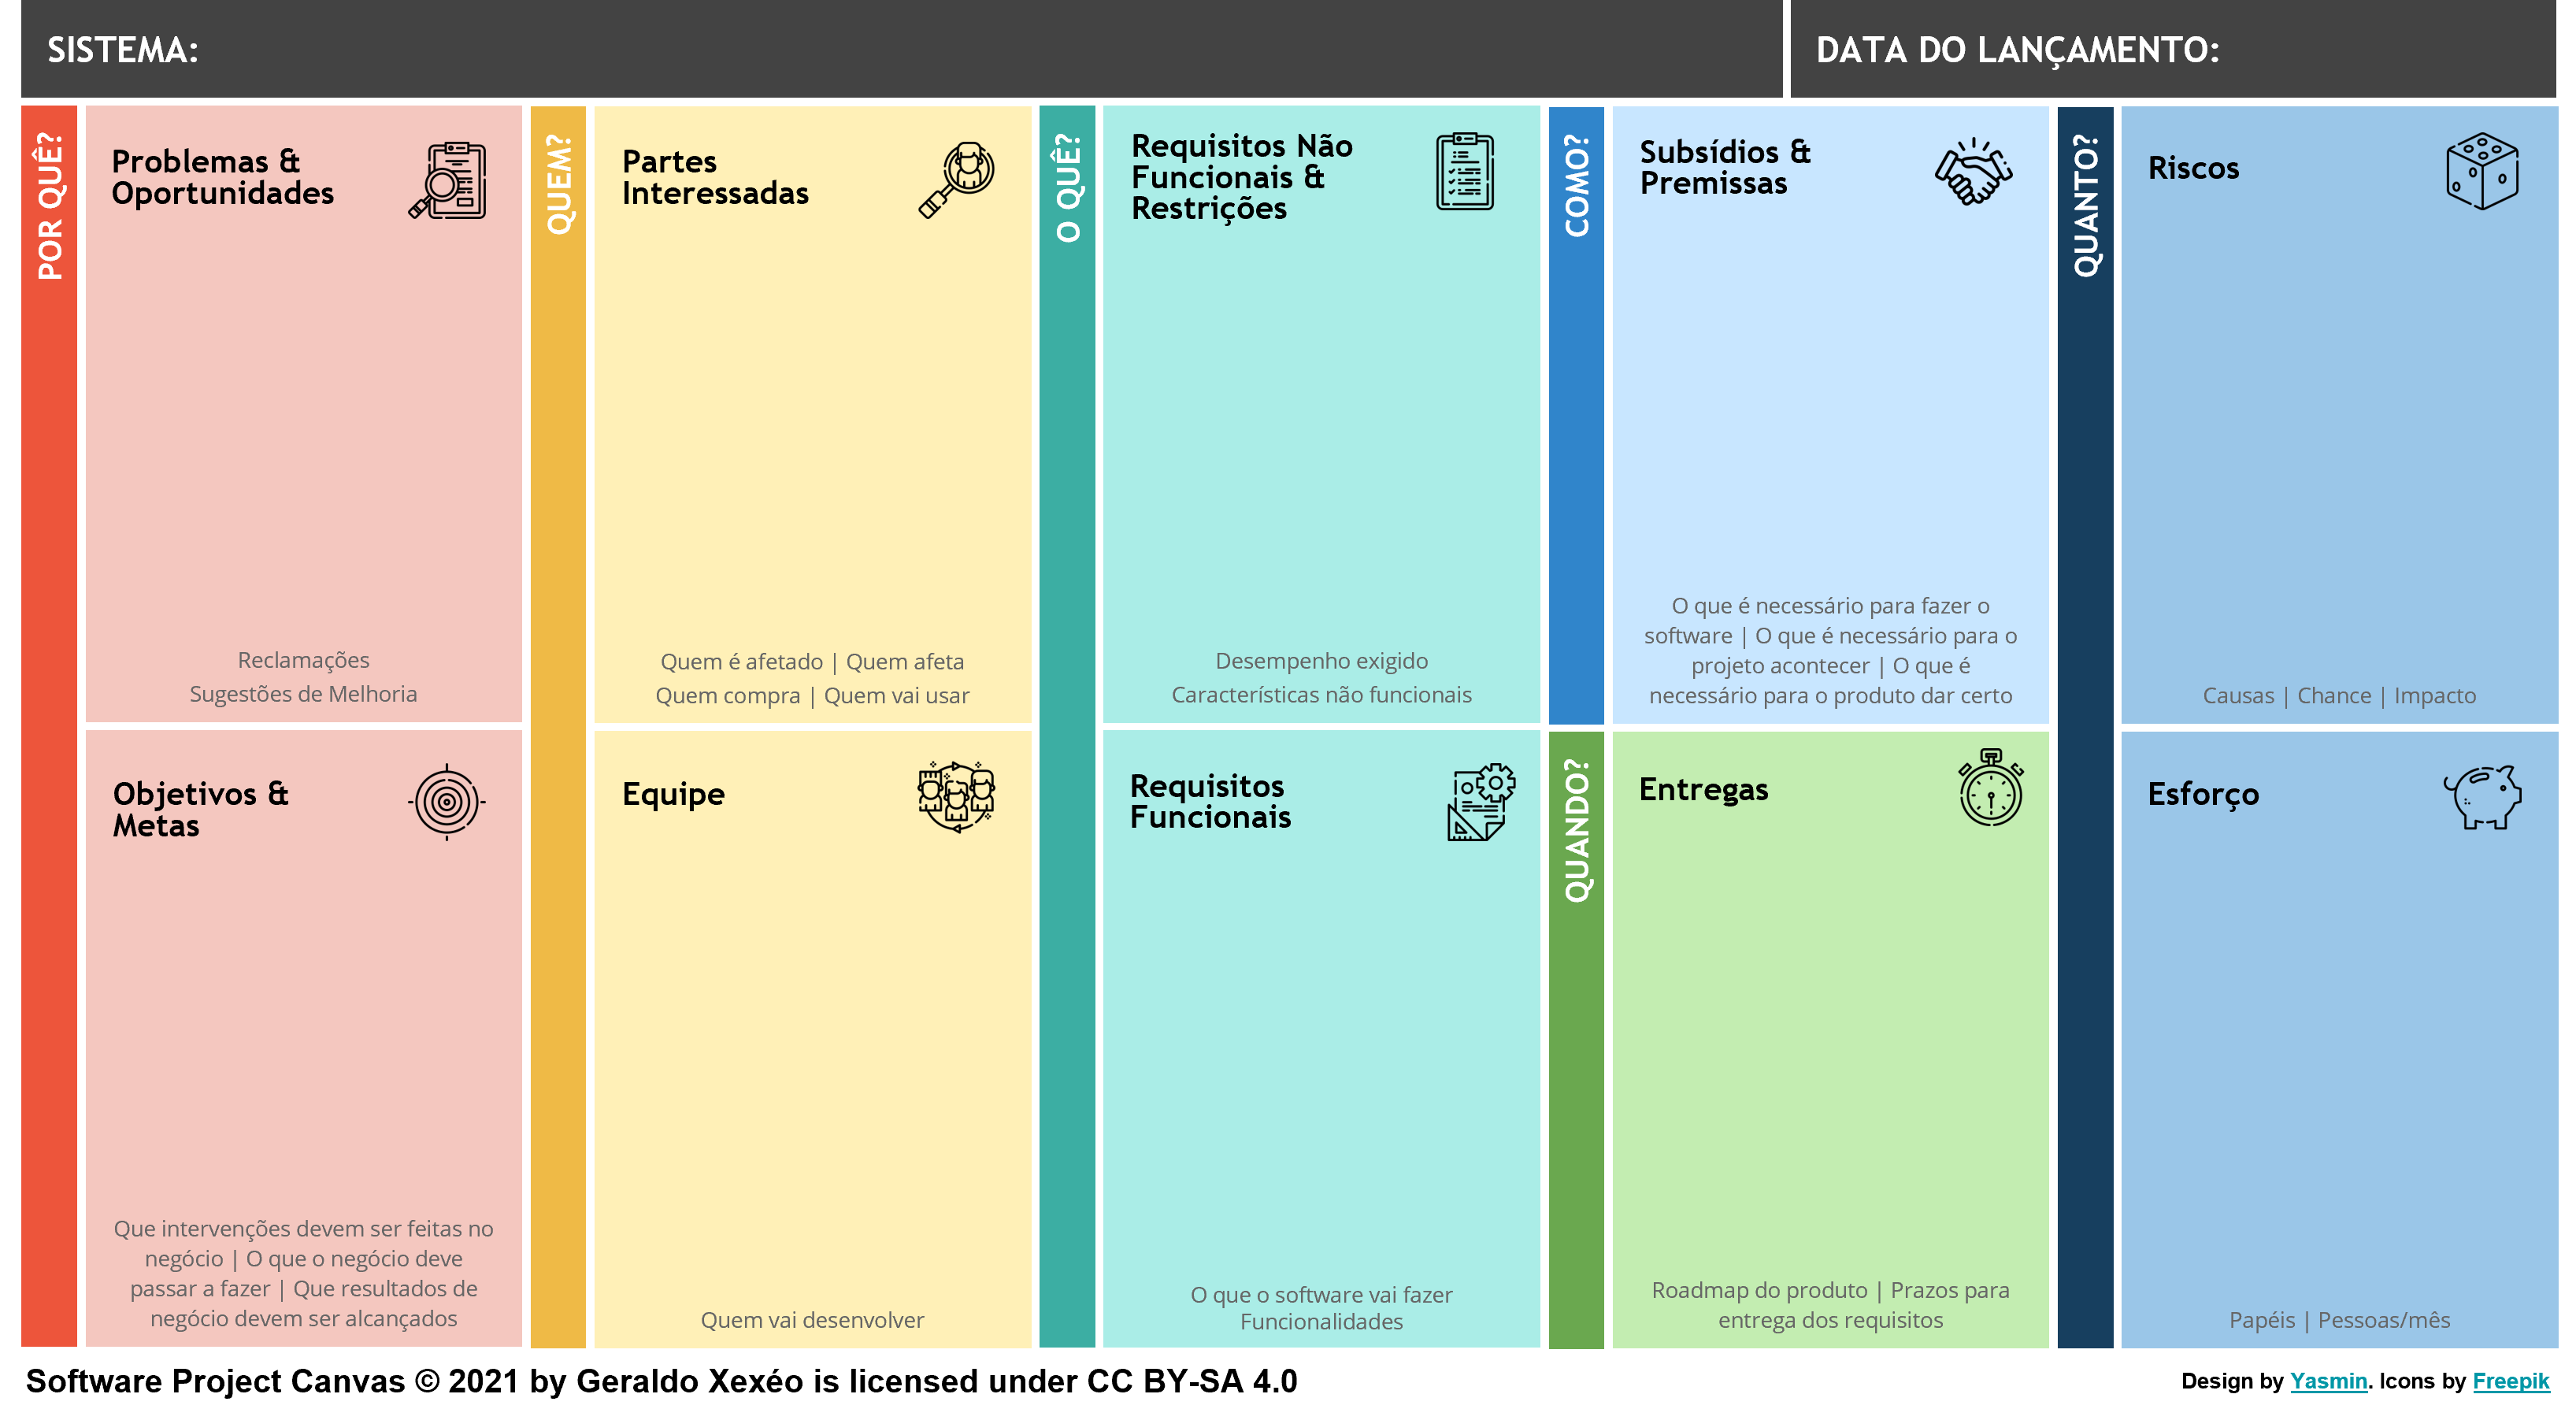
\includegraphics[width=0.9\textwidth]{imagens/alternativa3.png}
    \caption{Forma alternativa onde o projeto se inicia com os problemas e as partes interessadas. Fonte: imagem do autor.}
    \label{fig:alter3}
    \end{subfigure}
    \caption{Desenhos alternativos, que levam a processos alternativos para a fase de Conceber Projeto.}
    \label{fig:alternativas}
\end{figure}

Outra situação comum é temos como demanda inicial o "O quê". Nesse caso, não é recomendável começar pelos requisitos, mas sim pelos Problemas ou pelas Partes interessadas, para garantir uma melhor elicitação dos verdadeiros requisitos do projeto.



\subsection{Verificar Proposta}

A segunda atividade do processo tem como objetivo verificar a correção do \textit{Software Project Canvas} que será apresentado para validação na organização e com as outras partes interessadas.

Nessa fase, os participantes da reunião passam a se preocupar com a correção local e global do canvas, buscando garantir que ele apresenta um projeto coeso, racional e viável. 

Para isso, além de verificações \textit{ad-hoc}, é possível seguir um \textit{check-list} apresentado a seguir.
\begin{outline}
    \1 Verificações para os \textit{post-its}
    \2 Todo \textit{post-it} é claro e pode ser entendido por qualquer leitor ou parte interessada?
    \2 Todo \textit{post-it} está no quadro a que deve pertencer?
    \1 Verificações para os quadros
    \2 Os quadros estão organizados de forma que grupos de \textit{post-its} representem ideias semelhantes e que a importância ou prioridade de cada \textit{post-it} dentro do quadro ou assunto esteja representada?
    \2 Todos os \textit{post-its} dentro de um quadro estão em um mesmo nível de abstração?
    \2 Existem, em um quadro, elementos que são um sub-grupo de outro elemento no quadro. Por exemplo, uma parte interessada pode ser ``governo federal'' e outra ``Ministerio da Educação''. Isso é realmente desejado?
    \1 Verificações para o canvas
    \2 Todo o canvas está no mesmo nível de abstração?
    \2 A linguagem é consistente entre os quadros e \textit{post-its}?
    \2 Todo problema e oportunidade está atendido por meio de um objetivo ou meta?
    \2 Todo objetivo, e meta, busca atender um problema ou oportunidade? 
    \2 Toda meta tem uma métrica?
    \2 Os requisitos funcionais e não-funcionais atendem o Por Que do projeto?
    \2 As partes interessadas estão envolvidas com algum por que ou algum requisito ou restrição do projeto?
    \2 Requisitos e entregas deixam as partes interessadas satisfeitas?
    \2 Os subsídios e premissas são suportados por alguma parte interessada?
    \2 A equipe consegue atender os requisitos e cumprir as entregas?
    \2 As entregas atendem o porquê do projeto?
    \2 Todo risco está associado a alguma premissa, entrega, requisito ou restrição?
    \2 Toda premissa tem um risco, ou o risco foi pelo menos avaliado e considerado nulo?
    \2 As estimativas são razoáveis para o projeto e deixam as partes interessadas satisfeitas?
\end{outline}

\subsection{Validação}

Ao completar a verificação do canvas, é necessário validar o projeto com outras partes da organização, principalmente, com as partes interessadas interessadas que possuem, simultaneamente, poder, urgência e legitimidade sobre o projeto\cite{mitchell_toward_1997}. Para isso, deve ser feito um documento inicial com a proposta do projeto, que pode ser uma cópia do próprio canvas.

Fora da reunião, então, o projeto é validado e possíveis \textit{feedbacks} podem ser trazidos ao grupo original para melhorar, refinar, modificar ou mesmo abandonar o projeto, caso tenham sido encontradas falhas irremediáveis.


Este método não define uma forma fixa de se fazer a validação. Inclusive, grupos diferentes em uma mesma organização podem usar formas diferentes de validação. Podem ser usados reuniões, workshops, questionários, entrevistas, etc. 

O resultado dessa validação também não é definido em formato, e depende muito do tipo e da qualidade do \textit{feedback} recebido. A partir do resultado, o grupo responsável por lançar o projeto pode decidir não fazer nada, fazer pequenos ajustes ou voltar a fase de concepção.

\subsection{Compartilhar Projeto}

Na última fase do planejamento o projeto é compartilhado com a organização. Novamente, a forma de fazer isso dependende do projeto, da organização e da parte interessadas sendo atingida.  Pode ser necessário criar um plano de projeto formal para aprovação final em uma reunião anual, ou criar documentos mais ligados a métodos ágeis, como uma  visão do projeto ou um \textit{backlog} do produto para equipe de desenvolvimento, ou uma notícia para o jornal de divulgação interna. 






\section{Conclusão}

Este artigo apresenta o \textit{Software Project Canvas} um novo canvas para o planejamento ágil de um projeto de software. Ele foi criado para ser usado em substituição a outros canvas destinados ao planejamento inicial de projetos em geral, que são menos adaptados a linguagem e a prática dos desenvolvedores de software. Para a sua  criação foram observados \ref{problems:total} dificuldades encontradas ao ensinar ou utilizar o \textit{Project Model Canvas}, que serviu de fonte de inspiração. As adaptações feitas visam facilitar a explicação e o uso, além de evitar perda de tempo com discussões que não adiantam a definição do projeto.

No futuro será feita uma avaliação do uso do canvas em sala de aula e em projetos de software, a fim de validar as modificações feitas.



\section*{Agradecimentos}

Agradeço a Yasmin pelo design final do \textit{Software Model Canvas} e aos alunos, como Eduardo Mangeli, e Marcus Parreira, que fizeram críticas e sugestões.

\printbibliography

\end{document}
